\documentclass{article}
\usepackage[utf8]{inputenc}
\usepackage{pgfplots}
\pgfplotsset{width=10cm,compat=1.9}
\usepackage{amsmath,amssymb,amsthm}
\usepackage{graphicx}
\usepackage{float}
\usepackage{blindtext}
\usepackage{hyperref}
\usepackage{verbatim}
\usepackage{gensymb}
\usepackage{enumerate}
\usepackage{xcolor}
\usepackage{graphicx}
\hypersetup{
    colorlinks=true,
    linkcolor=blue,
    filecolor=magenta,      
    urlcolor=cyan,
    pdftitle={Overleaf Example},
    pdfpagemode=FullScreen,
    }
\usepackage[slovene]{babel}

\setlength{\parindent}{0pt}
\setlength{\parskip}{4pt}

\newcounter{example}[section]
\newenvironment{example}[1][]{\refstepcounter{example}\par\medskip
   \noindent \textbf{Naloga~\theexample. #1} \rmfamily}{\medskip}

\newtheorem*{zgled}{Zgled}

\title{Funkcije}
\author{Bor Bregant}
\date{\vspace{-5ex}}

\begin{document}

\maketitle

Funkcija ali preslikava $f$ iz množice $A$ v množico $B$ je predpis, ki vsakemu elementu iz $A$ priredi natanko en element iz množice $B$.

\begin{zgled}
    Zapiši definicijsko območje, zalogo vrednosti, ničle, intervale naraščanja in padanja, konveksnost, konkavnost, sodost in lihost za $f(x)=\sqrt{x^2 -1}$ in $g(x)=\ln (x^2-2x-3)$. Se nekaj primerov o osnovnih pojmih
\end{zgled}

\section{Računanje s funkcijami}

\begin{enumerate}[i]
    \item Vsota $\left(f+g\right)(x)=f(x)+g(x)$
    \item Razlika $\left(f-g\right)(x)=f(x)-g(x)$
    \item Produkt $\left(f\cdot g\right)(x)=f(x)\cdot g(x)$
    \item Kvocient $\left(\frac{f}{g}\right)(x)=\frac{f(x)}{g(x)}$ za $g(x)\neq 0, \forall x\in D_g$
    \item Produkt s številom $\left(k\cdot f\right)(x)=k \cdot f(x)$
\end{enumerate}

\begin{zgled}
    Zapiši vsoto, razliko, produkt in kvocient funkcij na intervalu $[-3,4]$.
\end{zgled}

\begin{example}
    DN 569c, 576, 578ad
\end{example}

\subsection*{Kompozitum funkcij}

\begin{figure}[H]
    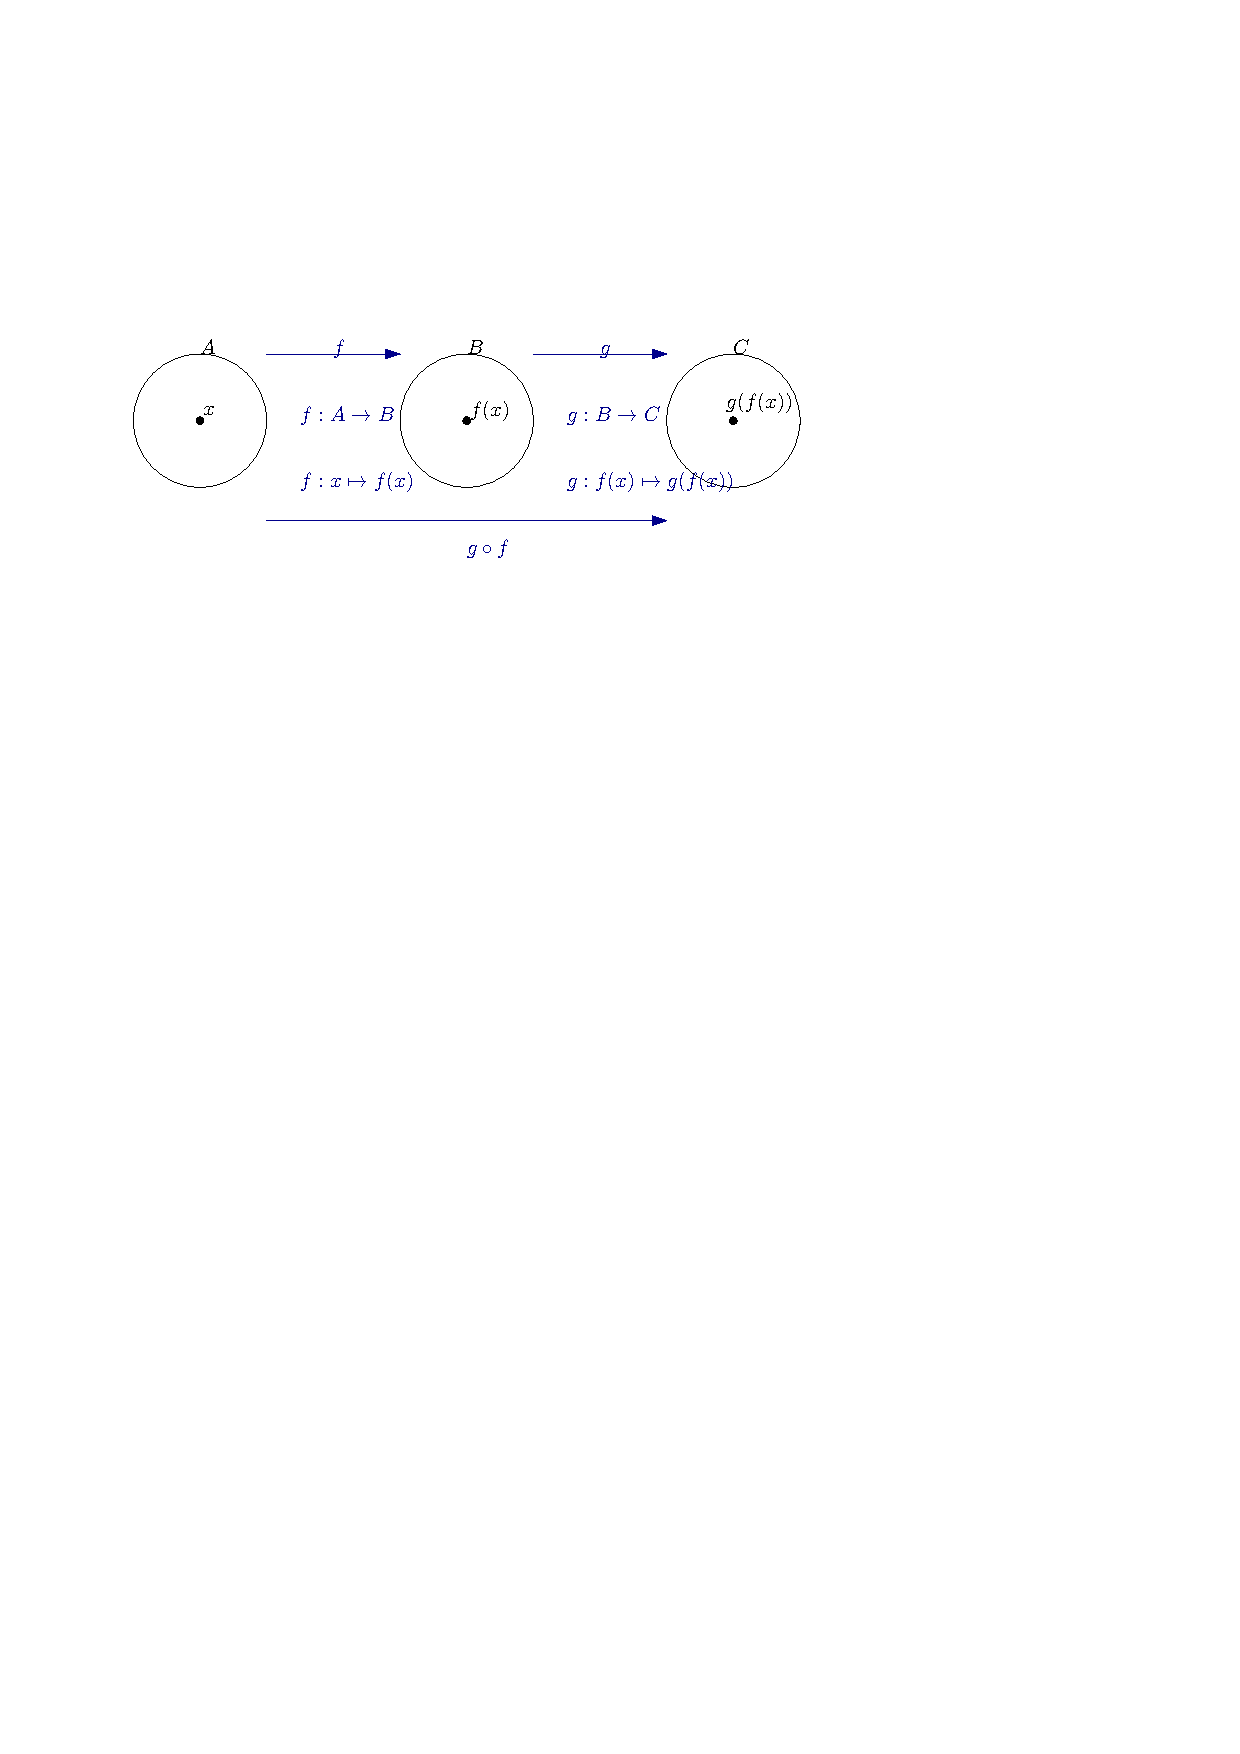
\includegraphics[width=0.7\textwidth]{kompozitum.pdf}
    \centering
\end{figure}

\begin{align*}
    & g\circ f: A\rightarrow C\\
    & g\circ f: x\mapsto g(f(x))\\
    & (g\circ f)(x)=g(f(x))\\
\end{align*}

\begin{zgled}
    Izračunaj $f\circ g$ in $g\circ f$ za $f(x)=\ln (x^2+2)$ in $g(x)=3x-1$ in pokaži, da ta operacija ni komutativna.
\end{zgled}

\begin{zgled}
    Poišči inverzno funkcijo za $f(x)=\sqrt[3]{x}+1$ in pokaži, da velja $(f\circ f^{-1})(x)=(f^{-1}\circ f)(x)=x$.
\end{zgled}
   
\begin{zgled}
    Dani sta funkciji $f(X)=2x-3$ in $g(x)=-x+2$. Za katera realna števila $x$ je $f(2x)=g(x)$ in za katera $f(-2)=g(x^2)$.
\end{zgled}

\begin{zgled}
    Dani sta funkciji $f(x)=3x+2$ in $g(x)=2x+n$. Za katera števila $n$ velja $f(g(x))=g(f(x))$?
\end{zgled}

\begin{zgled}
    Določi $k$, da bo $f(g(x))=g(f(x))$, kjer $f(x)=kx+3$ in $g(x)=kx-1$.
\end{zgled}

\begin{example}
    DN 574, 573ace, 587, 592ac
\end{example}

\section*{Limita in zveznost}

Funkcije, ki lahko narišemo z eno potezo so \textbf{zvezne}, sicer pa \textbf{nezvezne}.

Funkcija $f$ je zvezna v točki $a$, če in samo če:
\[\forall \varepsilon >0 \exists \delta >0: |x-a|<\delta \Rightarrow |f(x)-f(a)|<\varepsilon\]



\end{document}